%(BEGIN_QUESTION)
% Copyright 2009, Tony R. Kuphaldt, released under the Creative Commons Attribution License (v 1.0)
% This means you may do almost anything with this work of mine, so long as you give me proper credit

Identify the effects of the faults listed (considered one at a time) in this temperature control system:

$$\includegraphics[width=15.5cm]{i04019x01.eps}$$

\begin{itemize}
\item{} FTA-AI module resistor fails shorted
\item{} FTA-AI module resistor fails open
\item{} Ground wire falls off terminal TB40-8
\item{} Condensate valve left closed
\item{} Corroded wire connection at TB12-3
\item{} Cable 1 fails open
\item{} Cable 1 fails shorted
\item{} Cable 21 fails open
\item{} Cable 21 fails shorted
\end{itemize}

\vskip 20pt \vbox{\hrule \hbox{\strut \vrule{} {\bf Suggestions for Socratic discussion} \vrule} \hrule}

\begin{itemize}
\item{} A problem-solving technique useful for analyzing circuit faults is to first identify each component's function as either an electrical {\it source} or an electrical {\it load}.  Discuss and compare how these determinations aid in your analysis of component faults.
\item{} For those who have studied RTD temperature sensors, determine the effect of a short-circuit between terminals B and C on temperature transmitter
\end{itemize}

\underbar{file i04019}
%(END_QUESTION)





%(BEGIN_ANSWER)

\begin{itemize}
\item{} FTA-AI module resistor fails shorted: {\it temperature reads below-scale, may overheat as controller tries to increase temperature}
\item{} FTA-AI module resistor fails open: {\it temperature reads above-scale, will shut off all steam to the reactor}
\item{} Ground wire falls off terminal TB40-8: {\it may suffer extra noise voltage on temperature signal}
\item{} Condensate valve left closed: {\it reactor will not be able to heat after jacket fills with condensate}
\item{} Corroded wire connection at TB12-3: {\it steam control valve fails shut, causing reactor to cool down}
\item{} Cable 1 fails open: {\it steam control valve fails shut, causing reactor to cool down}
\item{} Cable 1 fails shorted: {\it steam control valve fails shut, causing reactor to cool down}
\item{} Cable 21 fails open: {\it temperature reads below-scale, may overheat as controller tries to increase temperature}
\item{} Cable 21 fails shorted: {\it temperature reads above-scale, will shut off all steam to the reactor}
\end{itemize}


%(END_ANSWER)





%(BEGIN_NOTES)


%INDEX% Basics, control loop troubleshooting: determining effect of specified fault(s)

%(END_NOTES)


